\begin{figure*}[t!hpb]
\caption{The LLOD Cloud}\label{f1}
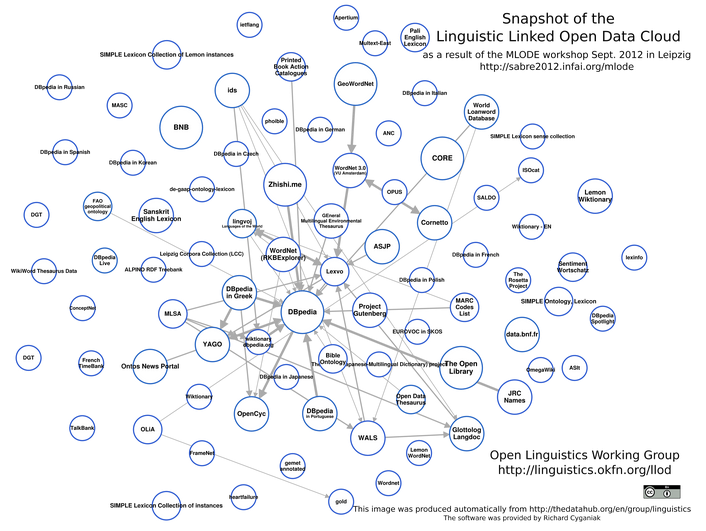
\includegraphics[width=15cm,keepaspectratio]{llod.png}
\end{figure*}

The Linguistic Linked Open Data (LLOD) cloud represents a very small but focused portion of the Semantic Web. It is specifically a so-called sub-cloud of the Linked Open Data cloud. The LLOD cloud is maintained by the Open Linguistics Working Group (OWLG),\footnote{\url{http://linguistics.okfn.org/}} which has three main goals for promoting openness in Linguistics: 

\begin{enumerate} 
	\item Promoting the idea of open linguistic data and resources
	\item Developing the means for the representation of open data
	\item Encouraging the exchange of ideas across different disciplines 
\end{enumerate}

Building an interoperable, linked data cloud is directly in line with these aims. The umbrella organization for the OWLG and other working groups, the Open Knowledge Foundation defines \textit{openness} as: ``A piece of content or data [that] is open if anyone is free to use, reuse, and redistribute it -- subject only, at most, to the requirement to attribute and share-alike.''\footnote{\url{http://opendefinition.org}} With this principle in mind, data from different resources and typological databases were converted into RDF and added to the LLOD cloud. Figure \ref{f1} provides an illustration of the current LLOD cloud and its contents.\footnote{This image was generated with software written by Richard Cyganiak. For an illustration of the entire LOD cloud, see: \url{http://lod-cloud.net}.}

The OWLG stipulates the following criteria for adding new resources to the LLOD cloud:

\begin{enumerate}
	\item data is resolvable through HTTP
	\item it is provided as RDF
	\item it contains links to another data set in the diagram 
	\item the entire data set must be available
\end{enumerate} 

At the time of writing, the cloud is in {\it draft} status, meaning that several of the resources may point only to resource metadata, even though the authors of these resources are committed to creating new links between to other linguistic datasets in the cloud. There are already many large and broad datasets that are linked in and across the LLOD cloud, including DBpedia, RDF versions of WordNet, Cornetto (Dutch WordNet), OpenCyc, and the Open Data Thesaurus. Linguistic-specific resources include data from typological databases like the World Atlas of Language Structures \citep{Haspelmath_etal2008}. There are metadata repositories, such as Glottlog/Langdoc, Lexvo and lingvoj that provide pertinent information about languages, such as bibliographic references for source materials, ISO codes for language name identifiers and language families, alternative language name indices, and information such as where the languages are spoken. Lastly, there are ontological resources that describe grammatical features of languages and their relationships, such as the General Ontology of Linguistic Description \citep{farrar2003linguistic}, and for terminology resolution ISOcat.\footnote{\url{http://www.isocat.org/}}
